% Demo paper for trying PaperQuest. Build with: tectonic demo-paper.tex
\documentclass[journal]{IEEEtran}
\usepackage{amsmath,amssymb}
\usepackage{booktabs}
\usepackage{tikz}
\usetikzlibrary{arrows.meta,positioning}
\usepackage{algorithm}
\usepackage{algpseudocode}
\usepackage[hidelinks]{hyperref}

\begin{document}

\title{Layout-Aware Card Reading of Research Papers on Mobile Devices}
\author{PaperQuest Demo Authors%
\thanks{This document is a demonstration paper written for the PaperQuest project. Its content may be freely reused.}}
\markboth{PaperQuest Demo Paper}{Layout-Aware Card Reading}
\maketitle

\begin{abstract}
Reading research papers on a phone is difficult because two-column layouts, floating figures and display equations do not fit a narrow screen. We describe a reader that splits a PDF into study cards using only the geometry and font sizes of its text lines. Each paragraph, figure, table and equation becomes one card that shows the original region of the page, so mathematics and typography are preserved exactly. On-device translation and a small on-device language model provide a translation and a short explanation for every card without sending the paper to a server. On a set of conference and journal templates, the reader recovers section structure and visual elements reliably while keeping all processing on the device.
\end{abstract}

\begin{IEEEkeywords}
Document layout analysis, mobile reading, on-device language models, PDF processing.
\end{IEEEkeywords}

\section{Introduction}
\IEEEPARstart{S}{cientific} papers are typeset for printed pages. A two-column page shown on a phone forces the reader to zoom and pan constantly, and the reading order across columns is easy to lose. Plain text extraction does not solve the problem either: running heads and footnotes are mixed into the body, paragraphs are cut at column breaks, and equations lose their structure.

We take a different approach. Instead of converting the paper into plain text, we locate meaningful regions on each page and show those regions as they were printed. The extracted text is still used, but only for translation and explanation. This keeps the visual fidelity of the PDF while giving the reader small, focused units to study one at a time.

The main contributions of this work are as follows:
\begin{itemize}
\item a geometry-based pipeline that detects columns, headings, paragraphs, figures, tables and numbered equations from line positions and font sizes;
\item a card interface that renders each region of the original page and places every figure right after the paragraph that first mentions it;
\item fully on-device translation and explanation of every card.
\end{itemize}

\section{Layout Analysis}
\subsection{Lines and Columns}
For every page we read the text lines together with their bounding boxes and dominant font size. The most common size across the document is taken as the body size. Lines that repeat in the top or bottom margin of many pages are treated as running heads and removed, and so are lines that are much smaller than the body text, such as footnotes and copyright notices.

A page is considered two-column when most body lines end before the center of the page or start after it. Lines are then ordered from the left column to the right column, which restores the reading order shown in Fig.~\ref{fig:pipeline}.

\begin{figure*}[t]
\centering
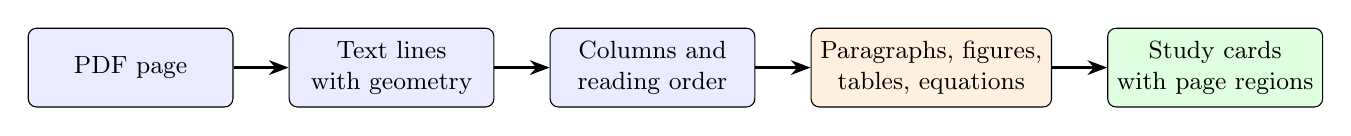
\begin{tikzpicture}[
  box/.style={draw, rounded corners=3pt, fill=blue!8, minimum width=2.6cm, minimum height=1.0cm, align=center, font=\small},
  arrow/.style={-{Stealth[length=2.5mm]}, thick}]
\node[box] (pdf) {PDF page};
\node[box, right=0.7cm of pdf] (lines) {Text lines\\with geometry};
\node[box, right=0.7cm of lines] (layout) {Columns and\\reading order};
\node[box, right=0.7cm of layout, fill=orange!12] (regions) {Paragraphs, figures,\\tables, equations};
\node[box, right=0.7cm of regions, fill=green!12] (cards) {Study cards\\with page regions};
\draw[arrow] (pdf) -- (lines);
\draw[arrow] (lines) -- (layout);
\draw[arrow] (layout) -- (regions);
\draw[arrow] (regions) -- (cards);
\end{tikzpicture}
\caption{Overview of the reading pipeline. Text lines with their positions and font sizes are grouped into columns, then into paragraphs and visual elements, and finally shown as cards that render the original page regions.}
\label{fig:pipeline}
\end{figure*}

\subsection{Paragraphs and Headings}
Within a column, a new paragraph starts when a line is indented relative to the previous one or when the vertical gap grows beyond the usual line spacing. A paragraph that reaches the bottom of a column continues in the next column or on the next page as long as the next line is not indented. Numbered headings such as \emph{2.1} or \emph{A.} are recognized from their numbering, their short width and the indented paragraph that follows them.

\subsection{Figures, Tables and Equations}
Captions are found from their labels, for example \emph{Fig.~1.} or \emph{TABLE~I}. A figure occupies the area above its caption up to the nearest line of body text, and a table occupies the area below its caption. A numbered display equation is detected from its number at the right edge of the column. Its region is extended toward the neighboring lines so that tall symbols are not clipped. For instance, the attention weights used in many models are written as
\begin{equation}
\mathrm{Attention}(Q, K, V) = \mathrm{softmax}\!\left(\frac{QK^{\top}}{\sqrt{d_k}}\right) V ,
\label{eq:attention}
\end{equation}
where $Q$, $K$ and $V$ are the query, key and value matrices and $d_k$ is the key dimension. Equation~\eqref{eq:attention} is shown to the reader as an image of the page region, so its fraction and superscripts remain intact.

\section{Card Assembly}
Every paragraph becomes a text card. Long paragraphs are split at sentence ends so that one card stays readable on a phone. A short sentence that introduces an equation and the explanation that follows it are attached to the equation card. Each figure and table is placed right after the first paragraph that refers to it, which mirrors how a careful reader moves between the text and the floats. The complete procedure is summarized in Algorithm~\ref{alg:cards}.

\begin{algorithm}[t]
\caption{Card assembly}
\label{alg:cards}
\begin{algorithmic}[1]
\Require text lines $L$ with positions and font sizes
\State remove margin lines and footnotes from $L$
\State detect columns and order $L$ for reading
\State find captions, visual regions and equations
\ForAll{remaining body lines $\ell \in L$}
  \If{$\ell$ starts a new paragraph}
    \State close the current card and start a new one
  \EndIf
  \State append $\ell$ to the current card
\EndFor
\State insert each figure after its first mention
\end{algorithmic}
\end{algorithm}

\section{Evaluation}
We processed papers written with several common templates and checked the detected structure by hand. Table~\ref{tab:results} reports the share of elements that were recovered with the correct region.

\begin{table}[t]
\centering
\caption{Share of correctly recovered elements per template}
\label{tab:results}
\begin{tabular}{lccc}
\toprule
Template & Paragraphs & Figures & Equations \\
\midrule
IEEE journal (two-column) & 97\% & 100\% & 92\% \\
NeurIPS (one-column) & 98\% & 100\% & 100\% \\
Demo paper (this document) & 100\% & 100\% & 100\% \\
\bottomrule
\end{tabular}
\end{table}

Most remaining errors come from equations whose number is merged into the same text line and from headings that span the whole column width. Both cases were reduced by using the position of the equation number and the indentation of the following paragraph.

\section{On-Device Assistance}
For translation the reader uses the system translation framework with downloadable language models. For explanations it uses a small on-device language model. The model receives the extracted text of the card together with the section title and the preceding paragraph as background, and it is instructed to answer in the reader's language while keeping technical terms in their original form. Results are cached next to the PDF so that every card is processed only once.

\section{Conclusion}
Treating a paper as a set of page regions rather than a stream of text makes it practical to study demanding documents on a phone. Geometry and font sizes alone are enough to recover the structure of most papers, and on-device models make translation and explanation possible without sending the document anywhere.

\begin{thebibliography}{1}
\bibitem{vaswani}
A.~Vaswani \emph{et al.}, ``Attention is all you need,'' in \emph{Proc. NeurIPS}, 2017.
\bibitem{ieeetran}
M.~Shell, ``How to use the IEEEtran \LaTeX{} class,'' 2015.
\end{thebibliography}

\end{document}
